\documentclass{article}

\usepackage[spanish]{babel}
\usepackage[utf8]{inputenc}
\usepackage[a4paper]{geometry}
\usepackage[pages=some]{background}
\usepackage{fontspec}
\usepackage[font=footnotesize]{caption}
\usepackage{xcolor}
\usepackage{hyperref}
\usepackage{url}
%%%%%%%%%%%%%%%%%%%%%%%%%%%%%%%%%%%%%%%%%%%%%%%%%%%%%%%%%%%%%%%%%%%%%%%%%%%%%%%%%%%%%%%%%%%%%%%%%%%%
\usepackage{graphicx}
\usepackage{float}
\usepackage{listings}
\usepackage{multicol}
%\usepackage{wrapfig}
%\usepackage{parskip}
%\usepackage{enumerate}
%\usepackage{fancyhdr}
%\usepackage[nottoc,numbib]{tocbibind}
%\usepackage{ulem}
%\usepackage{gnuplottex}
%\usepackage{circledsteps}
%\usepackage{pdfpages}
%\usepackage{amsmath}
%\usepackage{lipsum}



\graphicspath{{imagenes}}
\geometry{top=2.54cm, bottom=2.54cm, left=2.54cm, right=2.54cm}
\setmainfont{OpenSans}
\hypersetup{pdfborder={0 0 0}}
\definecolor{color_contenido}{RGB}{73, 208, 197}
\definecolor{color_estructura}{RGB}{133, 153, 0}
\definecolor{color_orilla}{RGB}{60, 255, 0}
\definecolor{color_fondo}{RGB}{253, 246, 227}
\definecolor{color_titulo}{RGB}{0, 122, 204}
\lstset{backgroundcolor=\color{color_fondo}, basicstyle=\footnotesize, captionpos=b, commentstyle=\color{gray}, extendedchars=true, firstnumber=1, frame=single, keepspaces=true, keywordstyle=\color{color_estructura}, numbers=left, numbersep=10pt, numberstyle=\footnotesize\color{black}, rulecolor=\color{color_orilla}, showstringspaces=false, stepnumber=2, stringstyle=\color{color_contenido}, tabsize=2, title=\lstname, breaklines=true}
\newfontfamily{\fuentetitulo}{Righteous}
\newfontfamily{\fuentetituloII}{Amarante}
\newcommand{\fr}{\fuentetitulo\color{black}}
\newcommand{\fn}{\fuentetituloII\color{black}}



\begin{document}

    \begin{titlepage}
        %\BgThispage\backgroundsetup{scale=1, color=black, opacity=0.2, angle=0, contents={\includegraphics[width=\paperwidth]{  }}}
        \vspace*{1cm}
        {\fr\fontsize{30pt}{10pt}\selectfont
        %%%%%%%%%%%%%%%%%%%%%%%%%%%%%%%%%%%%%%%%%%%%%%%%%%%%%%%%%%%%%%%%%%%%%%%%%%%%%%%%%%%%%%%%%%%%%%%%%%%%
        % T I T U L O %%%%%%%%%%%%%%%%%%%%%%%%%%%%%%%%%%%%%%%%%%%%%%%%%%%%%%%%%%%%%%%%%%%%%%%%%%%%%%%%%%%%%%
        \begin{center}
            UNIVERSIDAD AUTÓNOMA \\DE QUERÉTARO\\
        
            \begin{figure}[H]
                \centering
                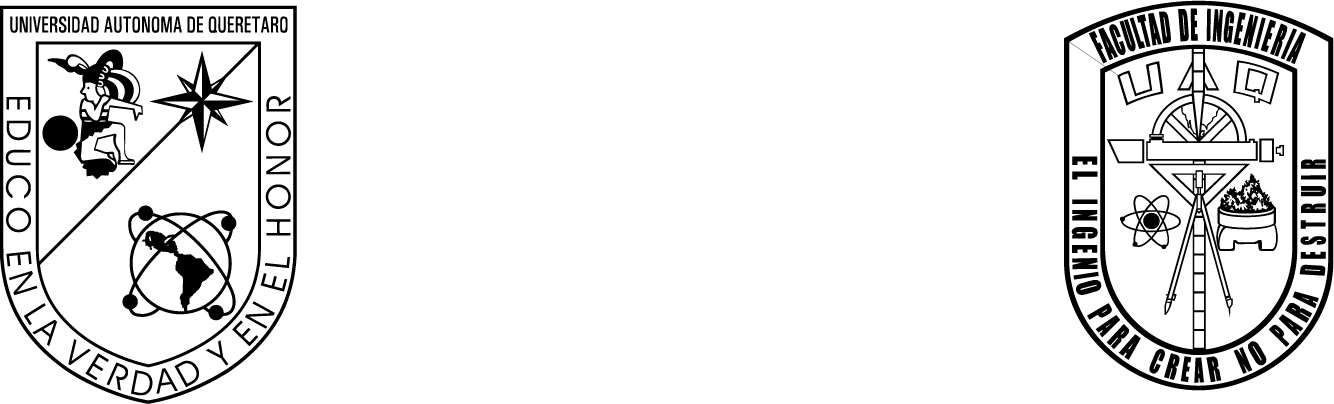
\includegraphics[height=5cm]{logos.png}
            \end{figure}
        %%%%%%%%%%%%%%%%%%%%%%%%%%%%%%%%%%%%%%%%%%%%%%%%%%%%%%%%%%%%%%%%%%%%%%%%%%%%%%%%%%%%%%%%%%%%%%%%%%%%
        %%%%%%%%%%%%%%%%%%%%%%%%%%%%%%%%%%%%%%%%%%%%%%%%%%%%%%%%%%%%%%%%%%%%%%%%%%%%%%%%%%%%%%%%%%%%%%%%%%%%
        \fontsize{20pt}{10pt}\selectfont
        \hspace*{2pc}
        %%%%%%%%%%%%%%%%%%%%%%%%%%%%%%%%%%%%%%%%%%%%%%%%%%%%%%%%%%%%%%%%%%%%%%%%%%%%%%%%%%%%%%%%%%%%%%%%%%%%
        % M A T E R I A %%%%%%%%%%%%%%%%%%%%%%%%%%%%%%%%%%%%%%%%%%%%%%%%%%%%%%%%%%%%%%%%%%%%%%%%%%%%%%%%%%%%
            FACULTAD DE INGENIERÍA\\
            ~\\ ~\\ ~\\
            Taller I\\
            Profesor: Ing. Gilberto Bustamante Balderas.\\
            Práctica No. 1.\\
            Enfocador de Telescopio.\\ ~\\ ~\\ ~\\
        \end{center}
        %%%%%%%%%%%%%%%%%%%%%%%%%%%%%%%%%%%%%%%%%%%%%%%%%%%%%%%%%%%%%%%%%%%%%%%%%%%%%%%%%%%%%%%%%%%%%%%%%%%%
        %%%%%%%%%%%%%%%%%%%%%%%%%%%%%%%%%%%%%%%%%%%%%%%%%%%%%%%%%%%%%%%%%%%%%%%%%%%%%%%%%%%%%%%%%%%%%%%%%%%%
        
        \fontsize{18pt}{10pt}\selectfont
        \begin{flushright}
            Alumnos: Colín Macías Luis Alberto,\\
            Ortíz Méndez José Santiago,\\
            Pizaña Juárez Luz Andrea,\\
            Sinecio Rivera Juliette.\\
            Fecha: \today
        \end{flushright} }
        \vspace*{\fill} 
    \end{titlepage}

    \newpage

    \tableofcontents
    \newpage

    \renewcommand{\chaptername}{Parte}

    %--------------------------------------------------------------------------------------------------%
    \section{Antecedentes.}
        Hace no más de medio año conseguí una cámara con la intención de acoplarla a mi telescopio para realizar fotografías. 
        Al acoplar una cámara a un telescopio (sobre todo si cuenta con montura ecuatorial) se tiene que equilibrar el peso extra que da la cámara. Una de las maneras más sencillas y baratas de equilibrar la cámara es colocarla de forma vertical con respecto al eje de ascensión recta.\\
        Eso presenta dos inconvenientes: El primero es una altura extra que dificulta el poder observar con el visor de la cámara (en caso de ser reflex) y el segundo es la disminución del campo visual con el nuevo ocular que pasa de aproximadamente 60º a únicamente 20º. Ambos problemas se pueden solucionar de una manera muy sencilla y disponible en la mayoría de las cámaras, el sistema Live View de Canon y análogos para otras marcas nos permite ver lo que verían nuestros ojos desde una pantalla que podemos colocar en una posición más cómoda.\\
        Con esos problemas resueltos nos surge un problema nuevo. Cuando vemos atrevés de un ocular nos es muy sencillo ocupar las manos para ajustar la perilla del enfoque y darnos una imagen nítida, pero qué pasa si no estamos viendo con un ocular y en cambio ocupamos una pantalla que puede estar lejos del alcance de la perilla. Nuestro proyecto viene para tratar de disminuir esta problemática.\\
    
    \section{Marco téorico.}
        Las placas micro-controladoras, muchas piezas electrónicas y en general las computadoras son capaces de utilizar el método de comunicación síncrono \textbf{Serial}, este método envía la información un byte a la vez. Al conectarse por un número limitado de cables solamente permite tener un dispositivo maestro por cada dispositivo esclavo.\\
        Una de las placas micro-controladoras que puede utilizar la comunicación serial es la Raspberry Pi Pico, que además de comunicarse de esa manera nos permite ejecutar programas Micropython que es una versión disminuida del famoso lenguaje de programación Python.\\

    \section{Objetivos.}
        El problema a resolver con este proyecto surge de la necesidad de enfocar con precisión un telescopio de manera semi-remota, intentando evitar en la medida de lo posible las interrupciones visuales como lo puede ser una vibración.\\

    \section{Metodología.}
        \subsection*{Explicación:}
            Para solucionar el problema debemos introducir una pieza capaz de emular el movimiento que nosotros realizamos con la mano al girar la perilla del enfoque. Como el movimiento que buscamos es un giro es que utilizaremos un motor a pasos, se pensó en alternativas como un servo motor y un motor de inducción pero ninguno cumplía con la necesidad que nos presenta el enfocador, pues debe de permitir dar más de una vuelta completa y ademas debe de ser preciso. Además de esas dos necesidades a cumplir debemos obtener un torque capaz de cargar el peso de la cámara, eso descarta el modelo 28byj-48 que es más barato, pero solo puede otorgarnos 0.34Kg/cm y nos deja con el modelo 17hs4401 que es capaz de otorgarnos 4Kg/cm.\\
            De nada nos sirve tener un movimiento que emule el nuestro si no somos capaces de transmitirlo a la pieza que necesitamos mover. Para transmitir el movimiento ocupamos un cople de motor comúnmente ocupado en modelismo.
            Para hacer que nuestro motor se mueva necesitamos mandarle las órdenes de movimiento y la corriente que necesita para funcionar para eso ocupamos el driver A4988 y la alimentación viene desde la micro-controladora, posteriormente se cambiará la fuente para evitar fallos y otorgar una mayor potencia al motor.\\
            Aquí entra nuestra tarjeta micro-controladora Raspberry Pi Pico que nos permite realizar el puente entre nuestro ordenador y nuestro driver del motor. Para hacer que funcione ocupamos el código \textbf{main.py}.\\
            Por último tenemos nuestra interfaz gráfica que corre dentro de un ordenador la cual nos permite enviar ordenes a la tarjeta microncotroladora la interfaz gráfica se encuentra en el archivo \textbf{enfocador.py}. Se puede ocupar cualquier ordenador siempre y cuando tenga instalado Windows (por el momento no hay compatibilidad con Linux), cuente con Python3 y tenga disponible un puerto USB para conectar la tarjeta.\\
        \subsection*{Código.}
            \subsubsection*{Código del programa instalado en la Raspberry Pi Pico.}
            \lstinputlisting[language=Python]{v3/main.py}
            \subsubsection*{Parte del código de la interfaz gráfica.}
            \lstinputlisting[language=Python, firstline=1, lastline=50]{v3/enfocador.py}
            En este código vemos la presencia de la clase Sender \cite{ref1}, esta es utilizada para comunicar la interfaz con la tarjeta.
        \subsection*{Conexiones.}
            \begin{figure}[H]
                \centering
                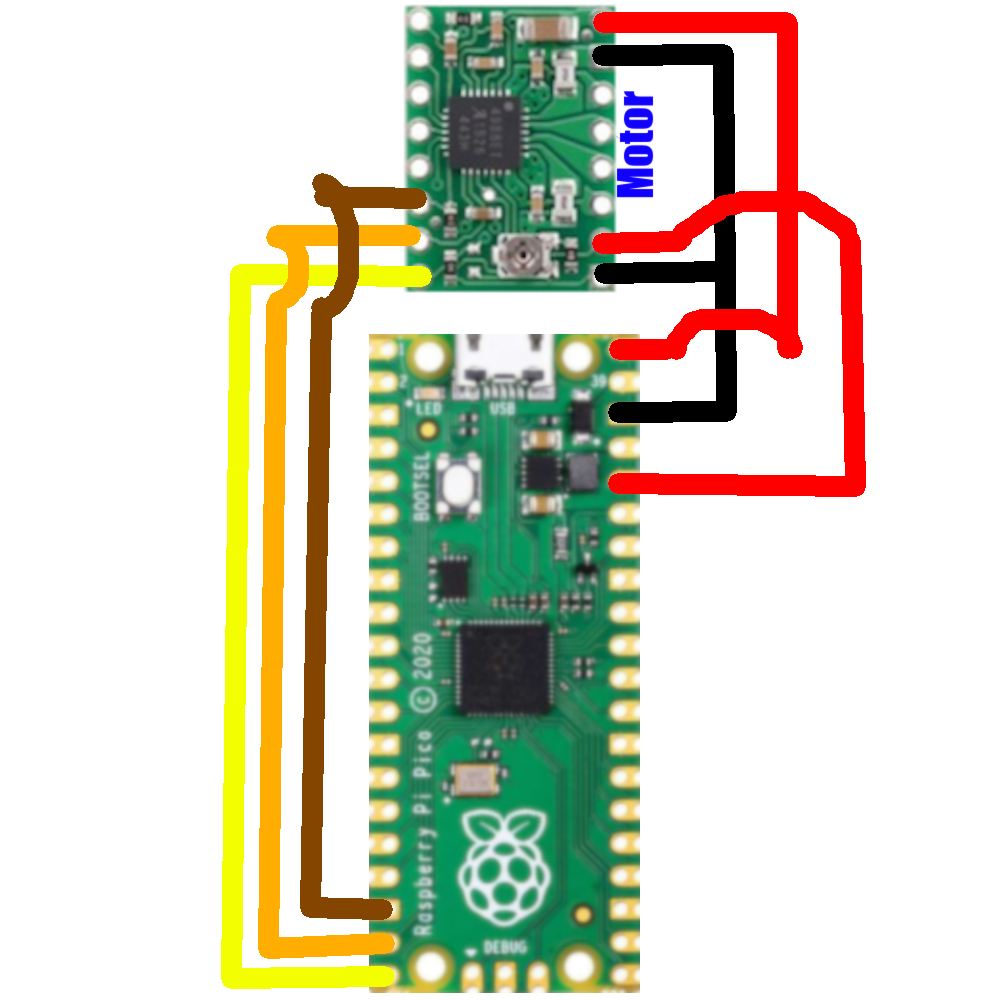
\includegraphics[width=\linewidth]{conexion.png}
                \caption{f. \cite{refi1} \cite{refi2} Esquema de la conexión.}
            \end{figure}
            Solo hay que mencionar que la entrada del motor debe ser en el mismo orden de los cables.
    \newpage
    \section{Resultados.}
        El proyecto nos permite realizar la función para la cual fue destinado, sin embargo no presenta la precisión tan exacta que se pensaba presentaría, para tener una mejor precisión será necesario cambiar la fuente del poder que va conectada al driver del motor y configurar el driver para que el movimiento sea más pequeño.
        \begin{multicols}{2}
            \begin{figure}[H]
                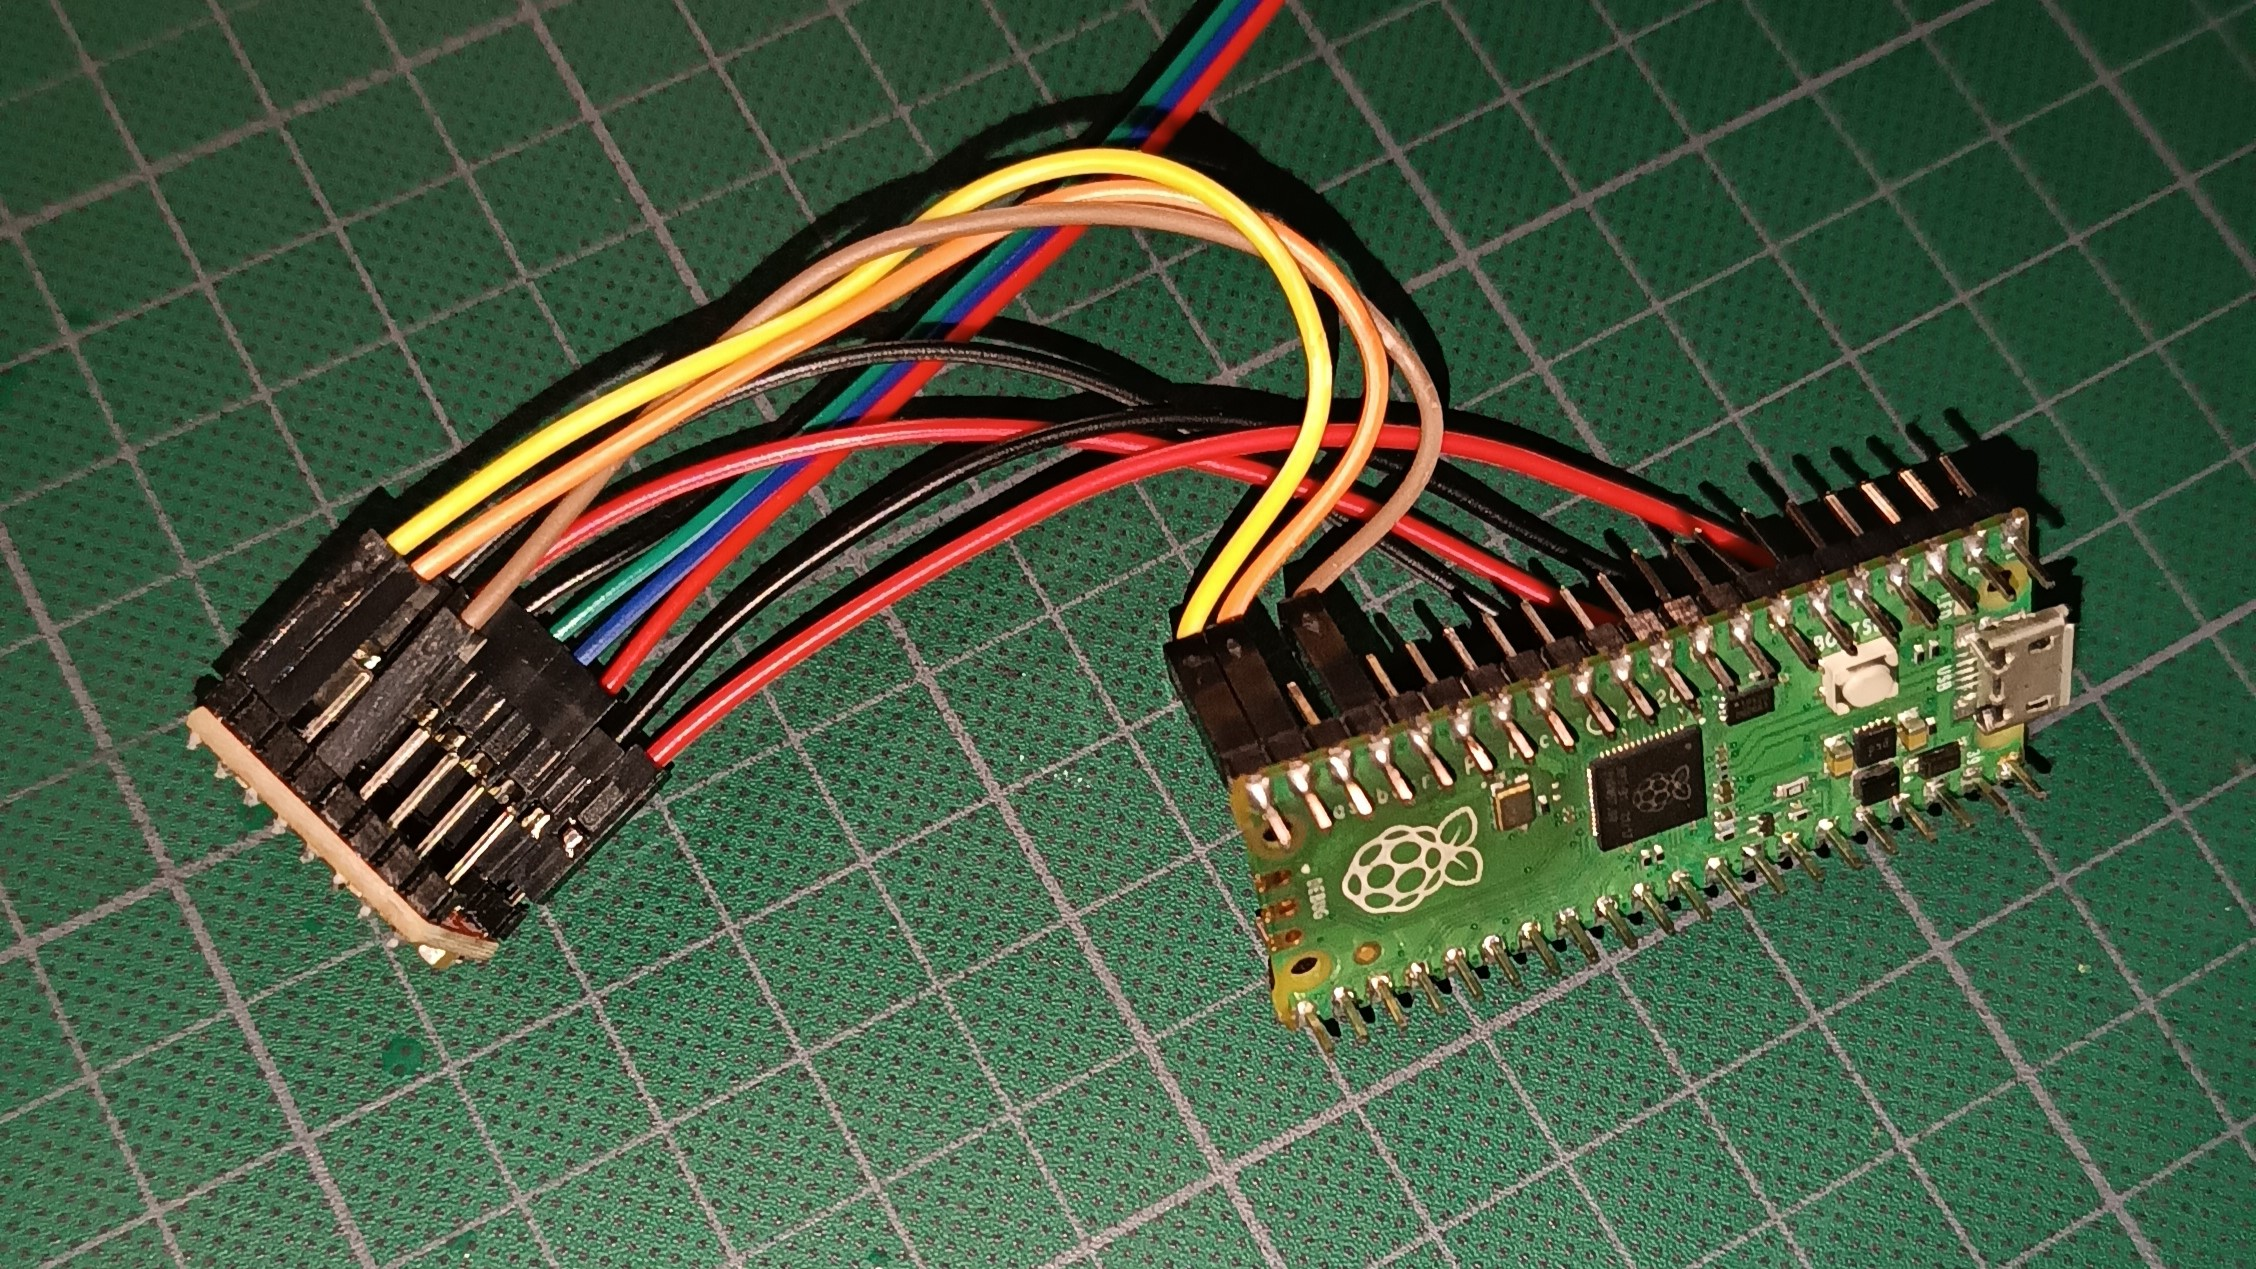
\includegraphics[width=\linewidth]{i1.jpg}
            \end{figure}
            \begin{figure}[H]
                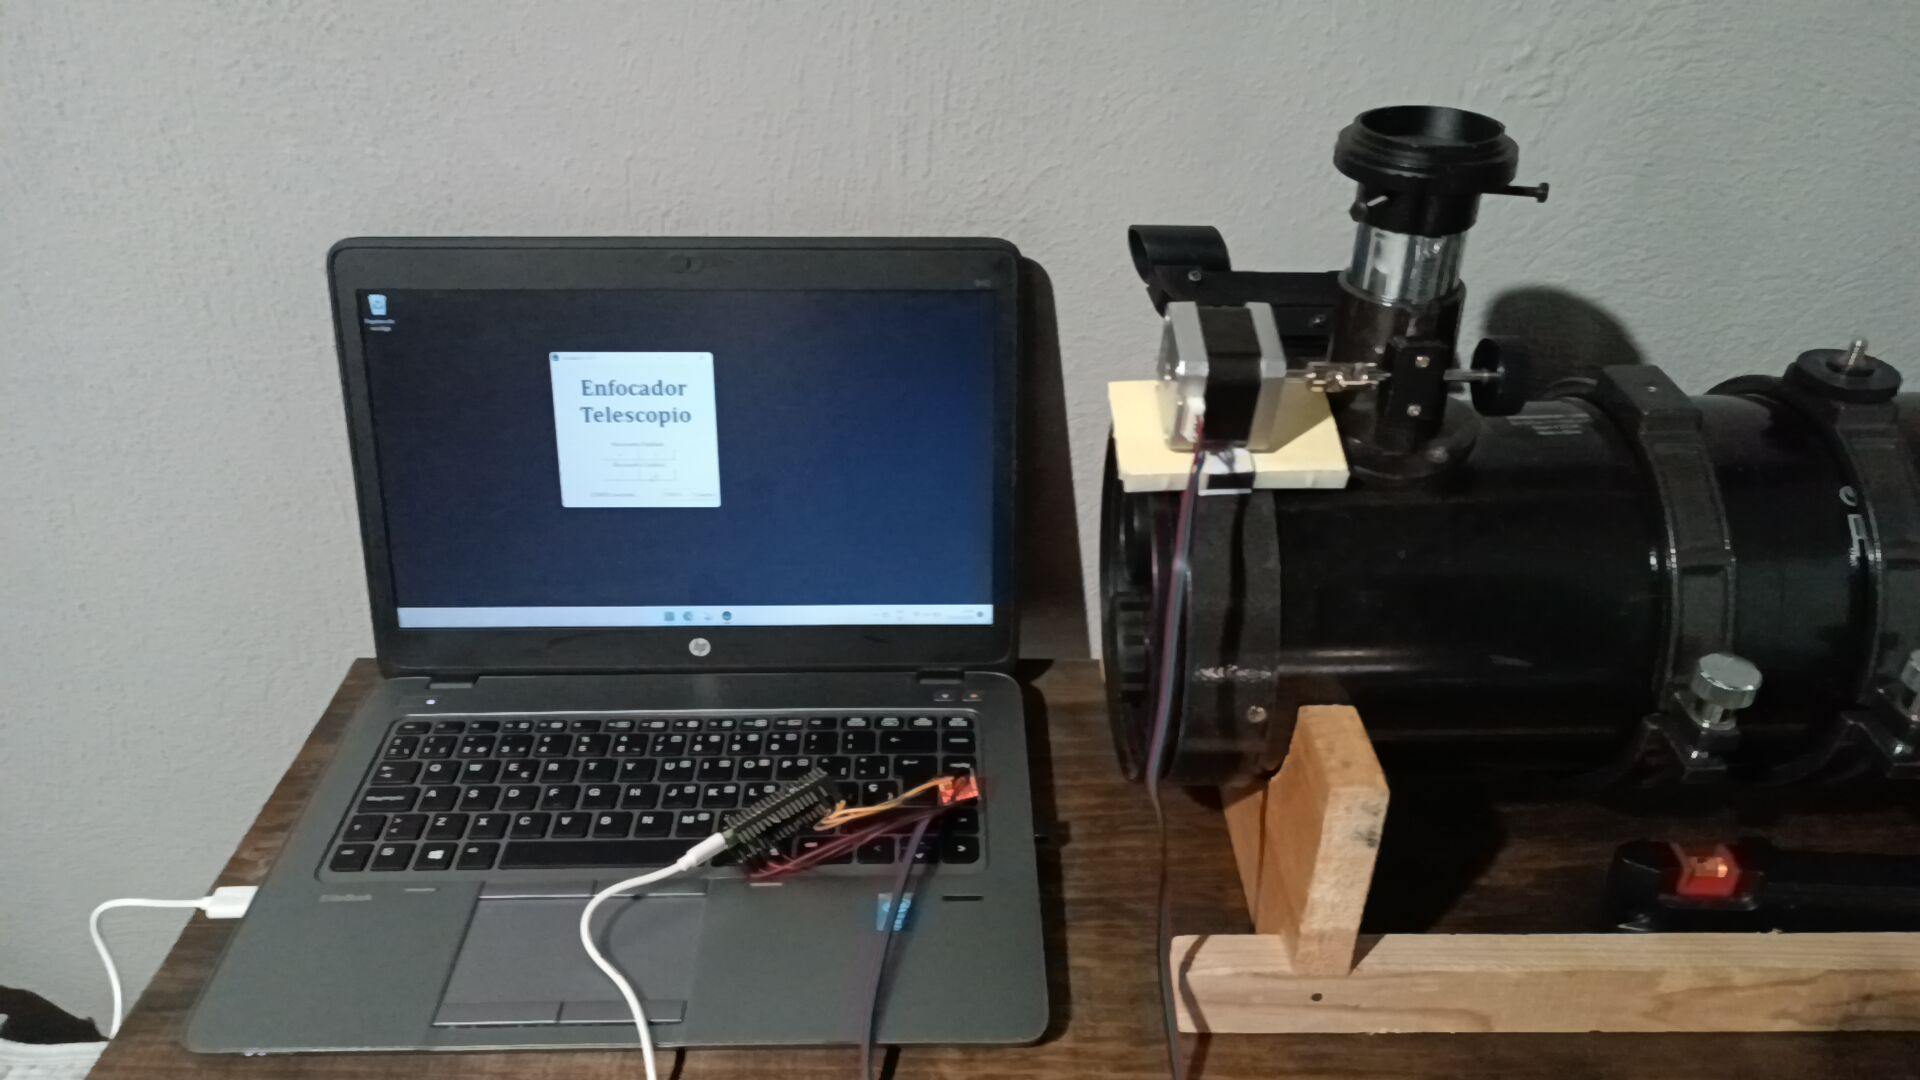
\includegraphics[width=\linewidth]{i2.jpg}
            \end{figure}
        \end{multicols}
        
    %--------------------------------------------------------------------------------------------------%
    \newpage
    \renewcommand{\bibname}{Referencias utilizadas.}
    \begin{thebibliography}{X}
        \bibitem{ref1} Cocking, R. (2022, 25 junio). Controlling a Raspberry Pi Pico remotely using PySerial. RAREblog. Recuperado 22 de mayo de 2022, de \url{https://blog.rareschool.com/2021/01/controlling-raspberry-pi-pico-using.html}
    	\bibitem{ref2} Colín, L. (s. f.). GitHub - CARALACM/Enfocador-Telescopio: Sirve para enfocar un telescopio. GitHub. \url{https://github.com/CARALACM/Enfocador-Telescopio}
        \bibitem{refi1} García, V. (s. f.). Esquema práctico general. [Esquema]. Electrónica Práctica Aplicada. \url{https://www.diarioelectronicohoy.com/blog/imagenes/2020/07/a4988.jpg}
        \bibitem{refi2} Raspberry Pi Pico. (s. f.). [Fotografía]. Tekno Movo. \url{http://teknomovo.com.mx/wp-content/uploads/2021/05/rasp-pico.jpg}
    \end{thebibliography}
    
\end{document}